%%%%%%%%%%%%%%%%%%%%%%% CHAPTER - 3 %%%%%%%%%%%%%%%%%%%%\\
\chapter{System Analysis and Architecture}
\label{C3} %%%%%%%%%%%%%%%%%%%%%%%%%%%%
\graphicspath{{images/}{Figures/}}
\noindent\rule{\linewidth}{2pt}
\textit{This Chapter delivers an in-depth analytical investigation of the existing campus placement paradigms, articulates the proposed architectural framework of Campus Agent, delineates hardware and software requirements, and details the overall system architecture, UML use case models, Data Flow Diagrams (Level 0 and Level 1), and data schema specifications.}
%%%%%%%%%%%%%%%%%%%%%%%%%%%%%%%%%%%%%%%%%%%%%%%%%%%%%%%%%%%%%%%%%%%%%%%%%%%%%%%%%%
\section{Existing System Analysis and Limitations} \label{S3.1}
In conventional university placement setups, the internship recommendation workflow is predominantly manual, fragmented, and asynchronous. Placement cells broadcast corporate notification PDFs and spreadsheet tables via broadcast email groups, messaging channels, or static institutional portals. Students are required to download each circular, manually read complex eligibility clauses, compare them against their own credentials, and independently track submission deadlines.

This traditional approach suffers from several grave vulnerabilities:
\begin{enumerate}[label=\textbf{\arabic*.}]
	\item \textbf{Cognitive Overhead and Information Fatigue:} Students are overwhelmed by dozens of overlapping notifications, resulting in missed deadlines and overlooked opportunities.
	\item \textbf{High Error Rate in Eligibility Self-Assessment:} Candidates frequently miscalculate semester credit requirements, confuse degree batch eligibility, or apply for opportunities whose durations violate university semester break regulations.
	\item \textbf{Zero Automated Skill Relevance Ranking:} Circulars are broadcast indiscriminately to all registered students without personalization. An AI/ML student receives notifications for mechanical CAD positions, while a Web Development enthusiast must manually search through hundreds of irrelevant postings.
	\item \textbf{Absence of Reassessment Tracking:} When a recruiter abruptly closes applications or raises CGPA cutoffs, no mechanism notifies previously eligible candidates of their updated status or suggests viable alternative openings.
\end{enumerate}

%%%%%%%%%%%%%%%%%%%%%%%%%%%%%%%%%%%%%%%%%%%%%%%%%%%%%%%%%%%%%%%%%%%%%%%%%%%%%%%%%%
\section{Proposed System Framework} \label{S3.2}
The proposed \textbf{Campus Agent} system re-engineers the campus internship discovery lifecycle into an intelligent, autonomous, and fully deterministic software platform. The key design tenets of the proposed framework include:
\begin{itemize}
	\item \textbf{Two-Stage Deterministic Engine:} Completely separates hard eligibility filtering (programme, year, CGPA, duration, commencement date) from soft relevance scoring (exact skill, partial skill, and domain alignment).
	\item \textbf{Automated Resume Ingestion:} Employs an integrated \texttt{pypdf} text mining pipeline to extract candidate skills, domain interests, academic programmes, cohort years, and CGPAs with zero manual typing.
	\item \textbf{Auditable Shortlist Reassessment Protocol:} Automatically generates a dynamic transition table detailing removed opportunities and promoting reconsidered alternatives when placement parameters shift.
	\item \textbf{Integrated Candidate Preparation Suite:} Bridges opportunity discovery with active interview preparation through What-If parameter simulation, drag-and-drop Kanban application tracking, and automated technical mock interview evaluation.
	\item \textbf{Autonomous Multi-Agent Scraper:} Extends the internal placement pool by harvesting active listings across 20+ top enterprise career portals using fast LLM semantic parsing and smart local NLP fallbacks.
\end{itemize}

%%%%%%%%%%%%%%%%%%%%%%%%%%%%%%%%%%%%%%%%%%%%%%%%%%%%%%%%%%%%%%%%%%%%%%%%%%%%%%%%%%
\section{System Requirements Specification} \label{S3.3}
The system has been engineered to run efficiently across standard consumer computing hardware and multi-platform environments.

\subsection{Hardware Requirements}
\begin{itemize}
	\item \textbf{Processor:} Modern x86-64 or ARM64 multi-core CPU (Intel Core i3/i5/i7, AMD Ryzen, or Apple Silicon).
	\item \textbf{Primary Memory (RAM):} 4 GB minimum (8 GB recommended for concurrent multi-agent scraping and browser rendering).
	\item \textbf{Storage:} 500 MB of free hard disk or SSD space for local dependencies, JSON datasets, and cached resume binaries.
	\item \textbf{Display:} $1280 \times 720$ minimum resolution ($1920 \times 1080$ Full HD recommended for optimal Kanban board visualization).
\end{itemize}

\subsection{Software Requirements}
\begin{itemize}
	\item \textbf{Operating System:} Microsoft Windows 10/11 (64-bit), macOS Monterey or newer, or modern Linux distributions (Ubuntu 20.04+).
	\item \textbf{Backend Runtime:} Python 3.8 to 3.11 with FastAPI, Uvicorn, Pydantic, and \texttt{pypdf}.
	\item \textbf{Frontend Runtime:} Node.js v16+ and npm 8+ with Vite build system and React 18.
	\item \textbf{Web Client:} Modern ECMAScript-compliant web browser (Google Chrome, Mozilla Firefox, Microsoft Edge, or Apple Safari).
\end{itemize}

%%%%%%%%%%%%%%%%%%%%%%%%%%%%%%%%%%%%%%%%%%%%%%%%%%%%%%%%%%%%%%%%%%%%%%%%%%%%%%%%%%
\section{Overall System Architecture} \label{S3.4}
The architecture of Campus Agent is structured as a decoupled, multi-tier system comprising a Client Presentation Layer, an Application Logic and Agent Layer, and a Persistence Storage Layer. The complete architectural blueprint is illustrated in Figure~\ref{f3.1}.

\begin{figure}[h!]
	\centering
	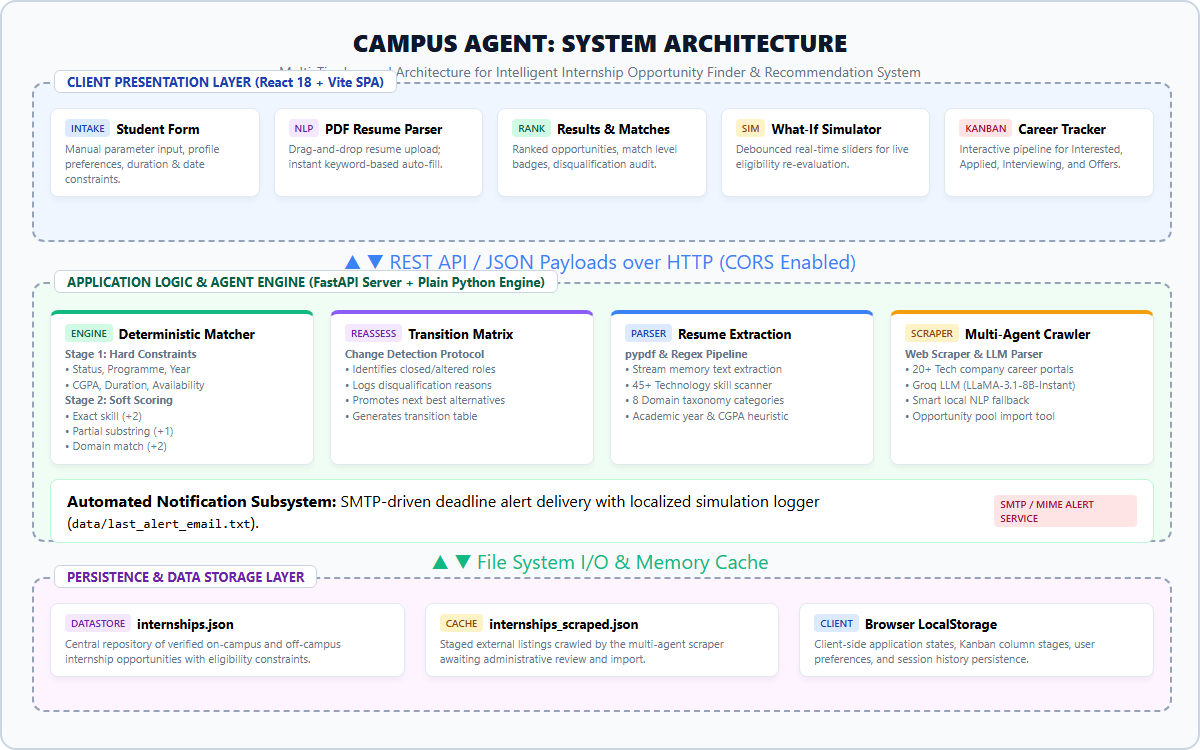
\includegraphics[width=\linewidth]{system_architecture.png}
	\caption{Overall Multi-Tier System Architecture of Campus Agent}
	\label{f3.1}
\end{figure}

As depicted in Figure~\ref{f3.1}:
\begin{enumerate}[label=\textbf{\arabic*.}]
	\item \textbf{Client Presentation Layer:} Implemented as a high-performance Single Page Application (SPA) using React 18 and Vite. It encapsulates five core user interface components: the Candidate Profile Intake Form, the PDF Resume Upload Dropzone, the Ranked Recommendations and Top Pick Card, the What-If Eligibility Parameter Simulator, and the Multi-Column Kanban Application Pipeline.
	\item \textbf{Application Logic and Agent Layer:} Powered by a high-throughput Python FastAPI server with asynchronous request processing and CORS middleware. It houses the deterministic two-stage matching engine (\texttt{agent.py}), the resume text mining pipeline, the dynamic shortlist reassessment matrix generator, the multi-agent web crawler (\texttt{scraper\_agent.py}), and the SMTP deadline notification service (\texttt{alerts.py}).
	\item \textbf{Persistence and Storage Layer:} Houses the primary verified internship database (\texttt{internships.json}), staged scraped listings (\texttt{internships\_scraped.json}), client-side application state storage via browser \texttt{LocalStorage}, and localized alert simulation files (\texttt{last\_alert\_email.txt}).
\end{enumerate}

%%%%%%%%%%%%%%%%%%%%%%%%%%%%%%%%%%%%%%%%%%%%%%%%%%%%%%%%%%%%%%%%%%%%%%%%%%%%%%%%%%
\section{Use Case Modeling} \label{S3.5}
To formalize the functional interactions between external human and autonomous actors and the Campus Agent platform, a UML Use Case Model was developed, as presented in Figure~\ref{f3.2}.

\begin{figure}[h!]
	\centering
	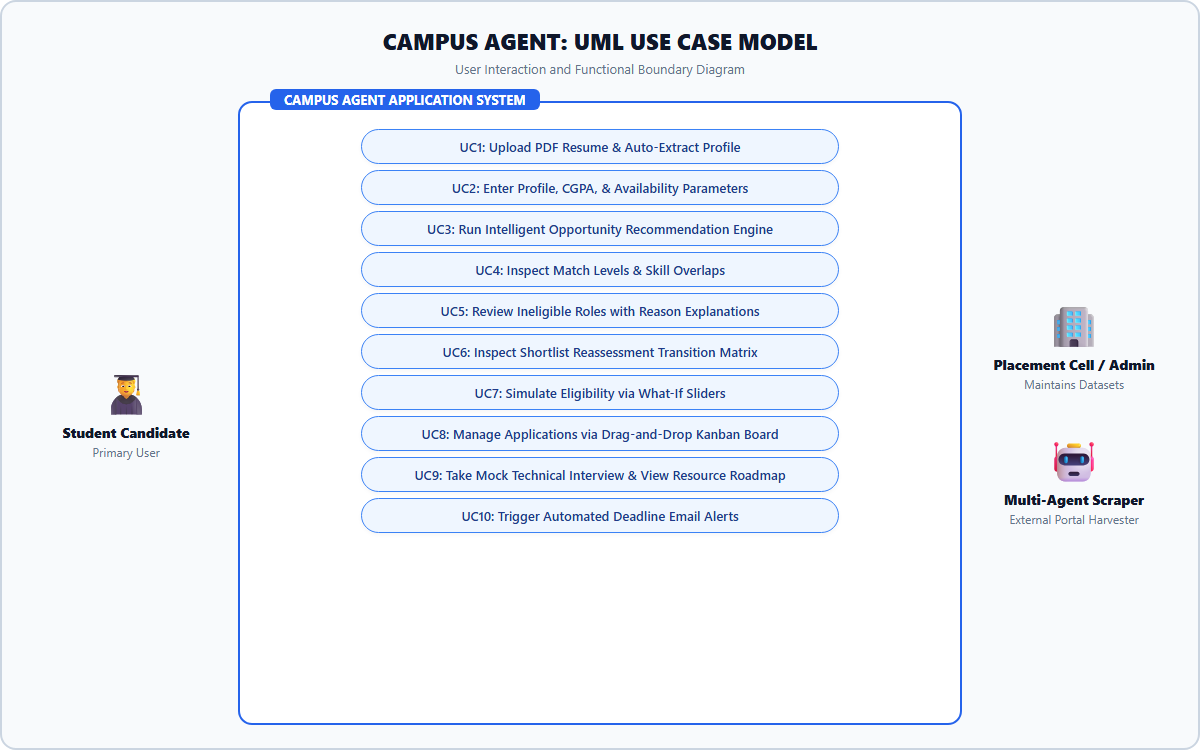
\includegraphics[width=0.92\linewidth]{use_case_diagram.png}
	\caption{UML Use Case Model Depicting Actor Interactions with System Boundaries}
	\label{f3.2}
\end{figure}

The primary actors interacting with the system include:
\begin{itemize}
	\item \textbf{Student Candidate (Primary Human Actor):} Ingests profile credentials manually or via PDF upload (UC1, UC2), triggers recommendation computation (UC3), inspects match scores and disqualification explanations (UC4, UC5), reviews shortlist transitions (UC6), tunes What-If sliders (UC7), tracks application stages on the Kanban board (UC8), and takes competency mock interviews (UC9).
	\item \textbf{Placement Officer / Administrator (Secondary Actor):} Curates verified on-campus opportunities, updates application statuses (e.g., toggling "Open" to "Closed"), and modifies eligibility criteria.
	\item \textbf{Multi-Agent Web Scraper (Autonomous Background Actor):} Crawls external enterprise career sites (UC10), extracts structured listings, and imports verified postings into the central database.
\end{itemize}

%%%%%%%%%%%%%%%%%%%%%%%%%%%%%%%%%%%%%%%%%%%%%%%%%%%%%%%%%%%%%%%%%%%%%%%%%%%%%%%%%%
\section{Data Flow Modeling} \label{S3.6}
The flow of information across system boundaries and internal functional transformations is modeled through Level 0 (Context Diagram) and Level 1 (Functional Decomposition) Data Flow Diagrams, as illustrated in Figure~\ref{f3.3}.

\begin{figure}[h!]
	\centering
	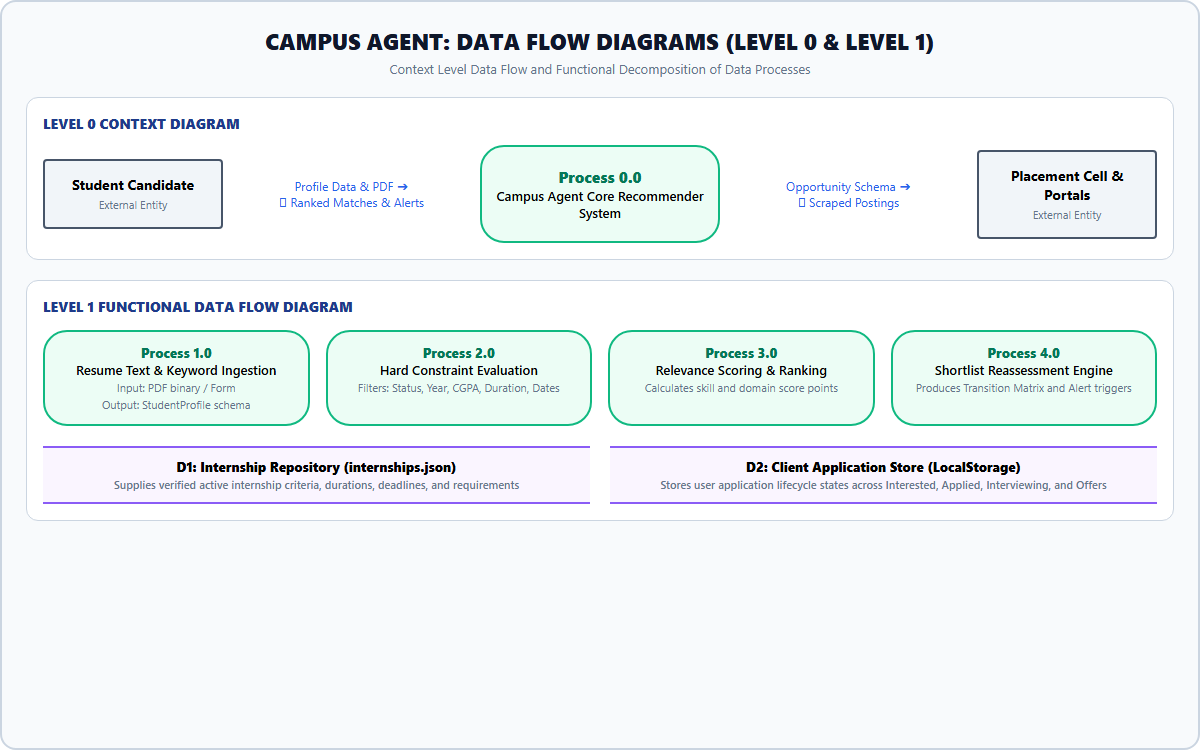
\includegraphics[width=\linewidth]{dfd_level0_level1.png}
	\caption{Level 0 Context Diagram and Level 1 Functional Data Flow Diagram}
	\label{f3.3}
\end{figure}

In the Level 0 Context Diagram:
\begin{itemize}
	\item The Student Candidate provides raw profile inputs or a binary PDF stream, receiving ordered recommendations, rejection audit trails, and deadline alerts.
	\item External Career Sites and Placement Cells feed opportunity schemas, receiving harvested records and application queries.
\end{itemize}

In the Level 1 Functional Decomposition:
\begin{itemize}
	\item \textbf{Process 1.0 (Resume Text \& Keyword Ingestion):} Transforms raw PDF streams into structured \texttt{StudentProfile} records.
	\item \textbf{Process 2.0 (Hard Constraint Evaluation):} Queries datastore D1 (\texttt{internships.json}), validating mandatory constraints and isolating disqualified opportunities.
	\item \textbf{Process 3.0 (Relevance Scoring \& Ranking):} Computes multi-term scoring functions, classifying match levels and sorting eligible items.
	\item \textbf{Process 4.0 (Shortlist Reassessment Engine):} Identifies state transitions, populating the dynamic transition matrix and triggering alert requests.
\end{itemize}

%%%%%%%%%%%%%%%%%%%%%%%%%%%%%%%%%%%%%%%%%%%%%%%%%%%%%%%%%%%%%%%%%%%%%%%%%%%%%%%%%%
\section{Database Schema and Entity Data Models} \label{S3.7}
Data structures within Campus Agent are governed by strongly-typed Pydantic schemas, guaranteeing runtime validation and strict schema conformity, as shown in Figure~\ref{f3.4}.

\begin{figure}[h!]
	\centering
	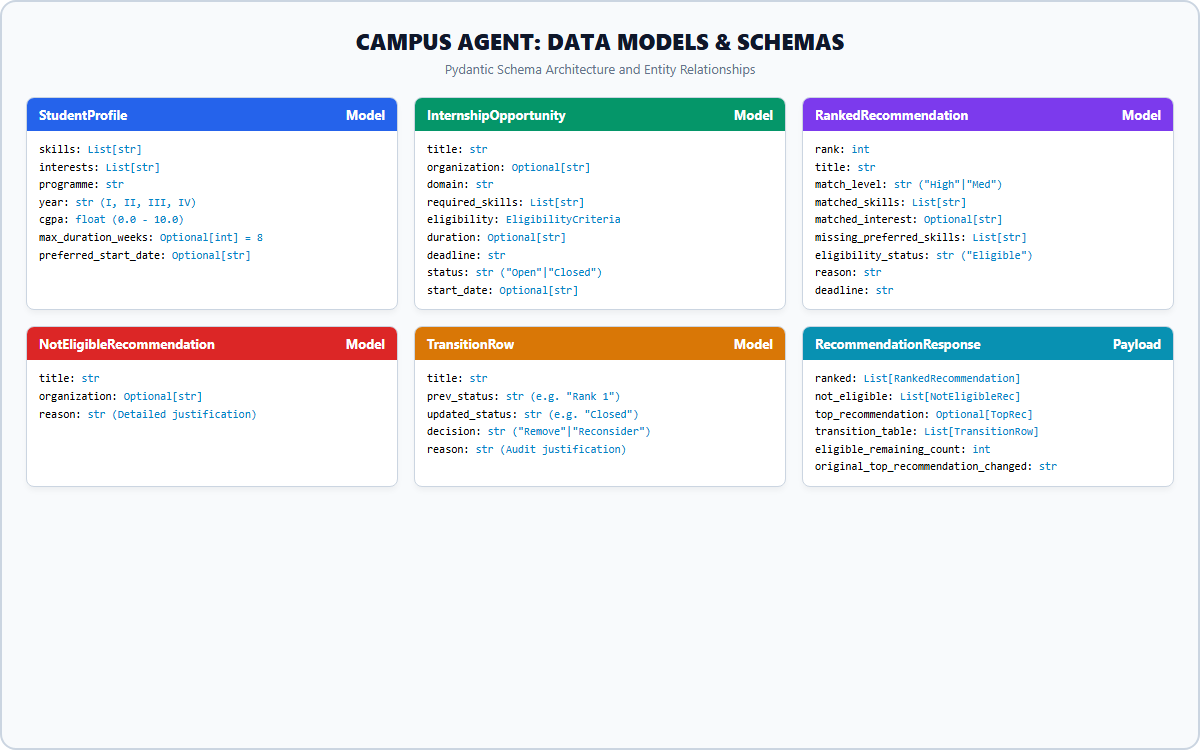
\includegraphics[width=\linewidth]{database_schema.png}
	\caption{Pydantic Schema Architecture and Entity Relationship Model}
	\label{f3.4}
\end{figure}

The principal data entities include:
\begin{itemize}
	\item \textbf{\texttt{StudentProfile}:} Encapsulates candidate skills, interests, academic programme, year of study, CGPA, maximum duration in weeks, and preferred availability date.
	\item \textbf{\texttt{InternshipOpportunity}:} Specifies title, organization, domain, required skills, nested \texttt{EligibilityCriteria} (programme, allowed years, minimum CGPA), duration string, deadline, status ("Open" or "Closed"), start date, and instructions.
	\item \textbf{\texttt{RankedRecommendation}:} Represents an eligible match with assigned rank, match level ("High", "Medium", "Low"), matched skills, domain overlap, missing preferred skills, reason sentence, and application links.
	\item \textbf{\texttt{NotEligibleRecommendation}:} Holds disqualified opportunity records paired with specific justification strings detailing all violated constraints.
	\item \textbf{\texttt{TransitionRow}:} Logs opportunity title, previous status (e.g., "Rank 1"), updated status (e.g., "Applications Closed"), agent decision ("Remove" vs. "Reconsider"), and audit rationale.
\end{itemize}

%%%%%%%%%%%%%%%%%%%%%%%%%%%%%%%%%%%%%%%%%%%%%%%%%%%%%%%%%%%%%%%%%%%%%%%%%%%%%%%%%%
\section{Summary} \label{S3.8}
This Chapter established the architectural foundation of Campus Agent, systematically comparing it against conventional placement methodologies, specifying hardware and software requirements, and illustrating the complete system architecture, UML use cases, Data Flow Diagrams, and Pydantic data schemas.
